{\color{gray}\hrule}
\begin{center}
\section{Pipeline and Implementation Details}
%\textbf{bla bla }
\end{center}
{\color{gray}\hrule}

\hfill

\subsection{General approach}

As depicted in the figure \ref{fig:general_pipeline}, our system will be subdivided into different modules each one designed to solve a specific step of the process:
\begin{itemize}[noitemsep]
\item Pre-processing: this module handles all which regards the image enhancement (denoising, light adjustement, etc...) and performs the background removal task;
\item Person Representation: this module performs pose estimation and the semantic segmentation of the person into their body parts;
\item Warping module: this module implements a geometric transformation that warps the fabric of the clothing item depending of the body shape and pose of the subject;
\item Try-On: this module generates a new image by composing the warped garment over the subject and should ensure the satisfaction of the requirements stated in the introduction section;
\item Image Retrieval: this module perform a content-based retrieval of the in-shop clothes, given a reference image.
\item Super-Resolution with Stable Diffusion: this module performs a zero-shot upscaling of the generated image of the Try-On module, based on the ControlNet architecture and some textual prompts.
\end{itemize}

Considering the e-commerce use case, during the inference, the customer inputs the target person image and the desired cloth image. The system selects the most similar in-shop cloth and then performs the virtual-try-on using these selected clothes.

\begin{figure*}[h]
\centering
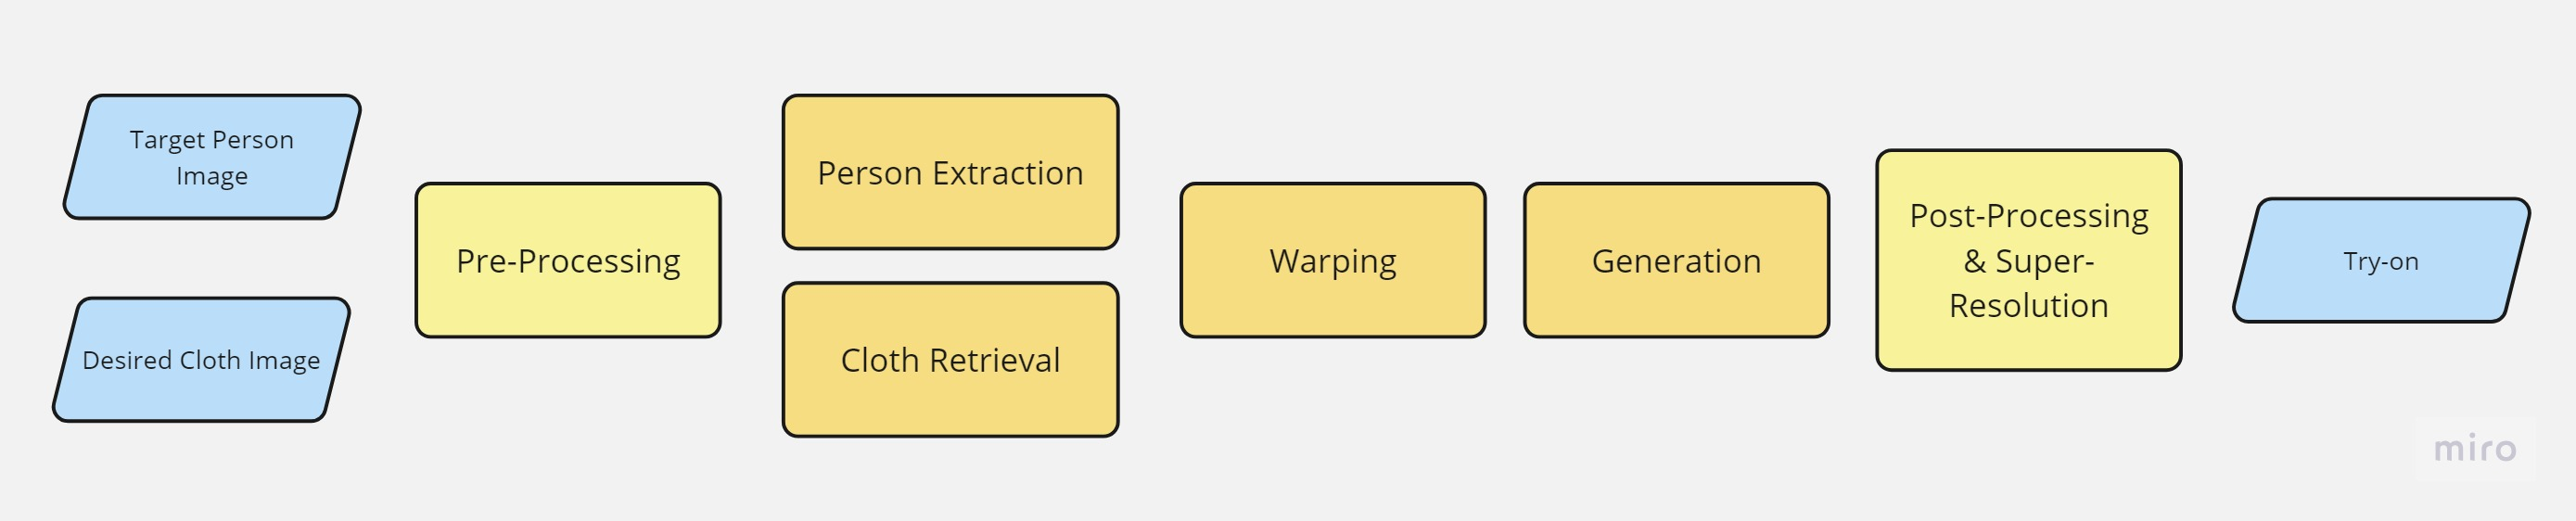
\includegraphics[width=\linewidth,height=100mm,keepaspectratio]{general_pipeline}
\caption{Overview of the pipeline}
\label{fig:general_pipeline}
\end{figure*}



In order to get across the inner workings of each module we will separate this section into subsections related to each one.


\subsection{Image Pre-Processing}
The system expects to receive two images: target person, desired cloth (it can be worn by a person or it can be cloth-only image). As the objective of the system is to be adaptable to dirty and noisy input images (so called "in-the-wild"), great care should be taken to clean such inputs.

\subsubsection{Image Enhancing}
As the objective of the system is to be adaptable to dirty and noisy input images, in the pre-processing phase great care should be taken to clean such inputs. As such the pre-processing module applies different methods of input refinement in sequence.

Firstly the image goes through a light adjustment procedure which entails contrast stretching with the following rule:
\begin{equation}
 I_o = (I_i - min_i)*((max_o - min_o)/(max_i - min_i)) + min_o
\end{equation}

then it goes through a denoising pass performed by a bilateral filter.



\subsubsection{Background Removal}
Given a person segmentation mask obtained by other means (see 3.3.2) we perform background removal creating a four-channel RGBA image and using the alpha channel and the mask to obtain only the foreground person. The algorithm can be found in \textit{preprocessing\_background\_removal.py}. In following example the background was designed to be salmon pink.

\begin{figure}[h]
\centering
\begin{tabular}{cccc}
\subfloat[Image]{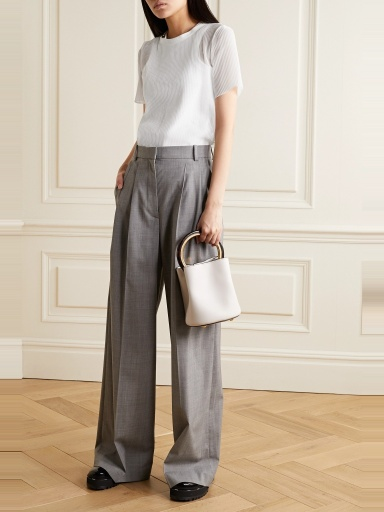
\includegraphics[width = 1.5in]{049433_0.jpg}} &
\subfloat[Mask]{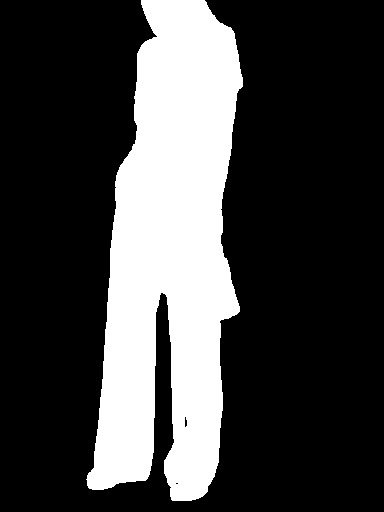
\includegraphics[width = 1.5in]{049433_0.png}} &
\subfloat[No background Image]{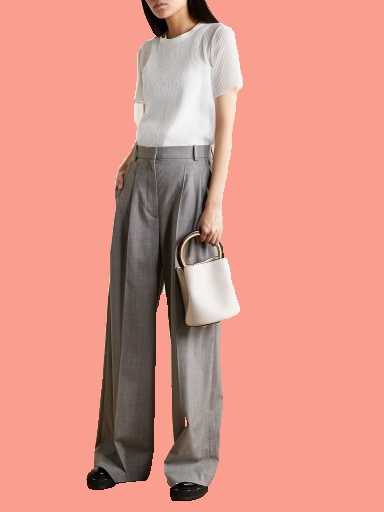
\includegraphics[width = 1.5in]{imgNoBG_0.jpg}} \\
\end{tabular}
\caption{Background Removal }
\end{figure}




\subsection{Person Representation Extraction}
This module performs pose estimation and the semantic segmentation of the person into their body parts. It is foundamental that the person representation is cloth-agnostic: the try-on task has to preserve the target person's information (face, hair, body shape and pose), while ignoring the worn cloth. We followed the CP-VTON \citep{CP-VTON} approach, so the person representation contains three components:

\begin{itemize}[noitemsep]
\item Pose Keypoints: the pose estimation contains information about the person pose. It follows the keypoints representation in OpenPose format. From the keypoints list, it is computed an 18-channel feature map with each channel corresponding to one human pose keypoint, drawn as an $11 \times 11$ white rectangle;

\item Body Shape: a 1-channel feature map of a blurred binary mask roughly covering different parts of human body;

\item Reserved Regions: an RGB image that contains the reserved regions that are not involved in thewarping or try-on phase (for instance feet, face, hair), detected using SCHP \cite{li2019selfcorrection} that generates the segmentation mask representing the human parsing of model body parts and clothing items. 
Our system was adapted to dynamically build different reserved regions images, depending on the different type of garment and the network module. 
\end{itemize}

\begin{figure}[h]
\centering
\begin{tabular}{cccc}
\subfloat[GMM Module Reserved Regions]{
\includegraphics[width = 1.5in]{parse_head_warping.png}} &
\subfloat[TOM Module Upper Body Reserved Regions]{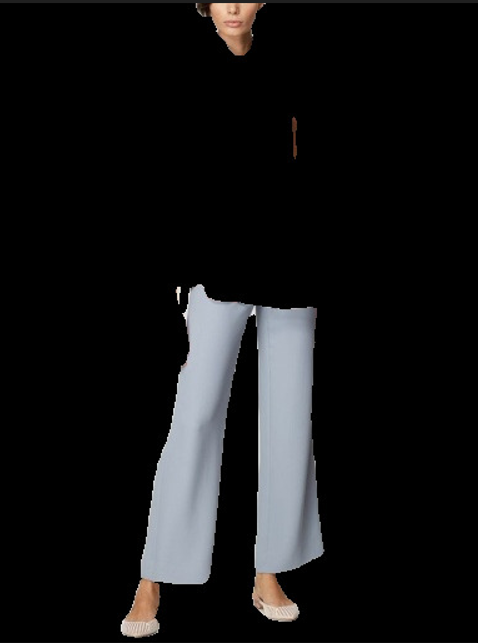
\includegraphics[width = 1.5in]{parseheadtom.png}} &
\subfloat[TOM Module Dresses Reserved Regions]{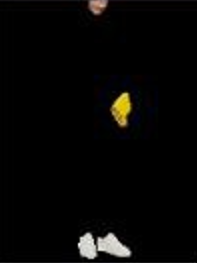
\includegraphics[width = 1.5in]{dress_parsehead.png}} \\
\end{tabular}
\caption{Different types of reserved regions}
\end{figure}

\subsubsection{Keypoints Extraction}

In order to extract pose-keypoints from a person image, we first attempted to use Openpose. Unfortunately, it did not seem to be compatible with our current environment. Model servers were down so the build continued to fail. As such, we adopted a solution based on the Detectron2 \cite{detectron2} keypoints extraction architecture (Model: \textit{COCO-Keypoints/keypoint\_rcnn\_R\_50\_FPN\_3x.yaml}. The keypoints were mostly compatible, but they were 17 instead of 18, and the indexes were placed in a different order. To solve this, we interpolated the missing keypoint and re-ordered them accordingly. This procedure can be found in \textit{detectron2\_scripts/d2.py}.


\subsubsection{Body-shape Mask Extraction}
 A simple script (\textit{preprocessing/mask\_generator.py}) extracts the binarized mask from the SCHP segmentation label map, flattening all body-parts labels into a unique person mask, separated from the background. 


\subsection{Cloth Mask Extraction}
As the DressCode dataset did not include the required cloth masks for the training and inference pipeline, we provided an iterative method to extract masks using Canny algorithm and other non-semantic image processing adjustments. Given a garment cloth image, the steps are the following:

\begin{itemize}
	\item Apply Canny algorithm to extract edges with upperthreshold = 100 and lowertreshold = 200.
	\item Apply a 5x5 squared Dilation kernel in order to concatenate disconnected lines.
	\item Apply findContours and drawContours methods, extracting only the most external outline of the image and filling it with white pixels.
	\item Checking if the mask is acceptable computing a white/black pixel ratio: if it is lower than a threshold, the mask generation has failed.
	\item If the mask has failed, a sharpening kernel k is applied to the original image and a second attempt is made.
\[
k=\begin{bmatrix}
		    0     & -1 & 0 \\
		    -1    & 5 & -1 \\
		    0     & -1  & 0 
		\end{bmatrix}
\]
	\item If the image has been sharpened, the final mask can appear to have rough borders. In order to improve the quality, a Median Blur filter is applied to the final mask image.
		
\end{itemize}

Eventually, this second-pass allowed to save about 20\% of the failed masks. The complete script can be found in \textit{preprocessing/cloth\_mask\_generator.py}.

\begin{figure}[h]
\centering
\begin{tabular}{cccc}
\subfloat[Original Image]{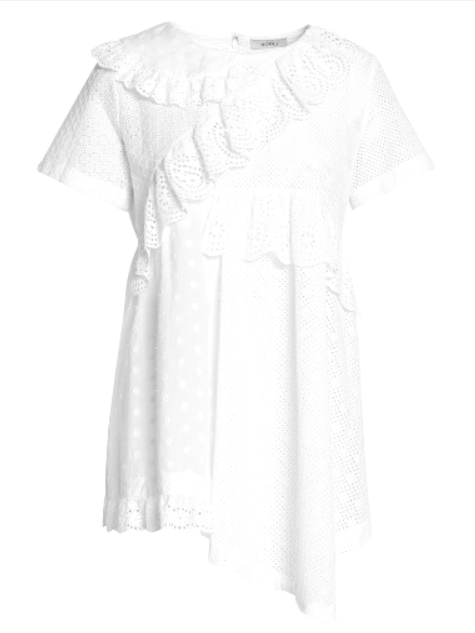
\includegraphics[width = 1.0in]{image1.png}} &
\subfloat[Canny Edges]{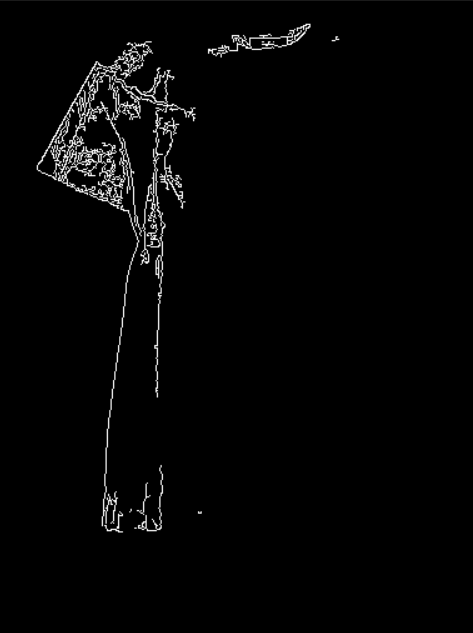
\includegraphics[width = 1.0in]{canny_edges.png}} &
\subfloat[Dilated Canny Edges]{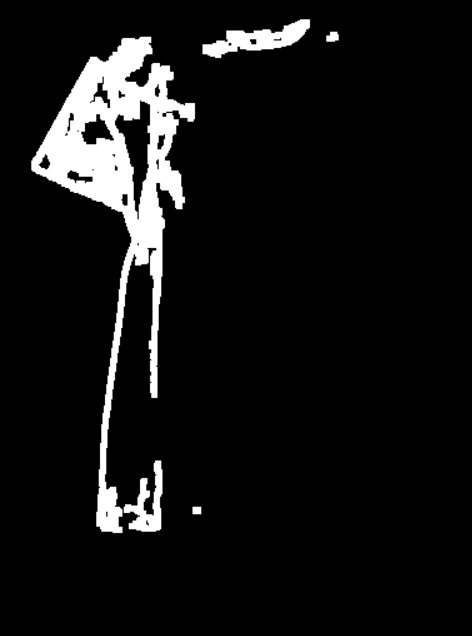
\includegraphics[width = 1.0in]{dilated_canny_edges.png}} &
\subfloat[Failed Mask]{
\includegraphics[width = 1.0in]{failed_mask.png}} \\
\subfloat[Image After Sharpening Kernel]{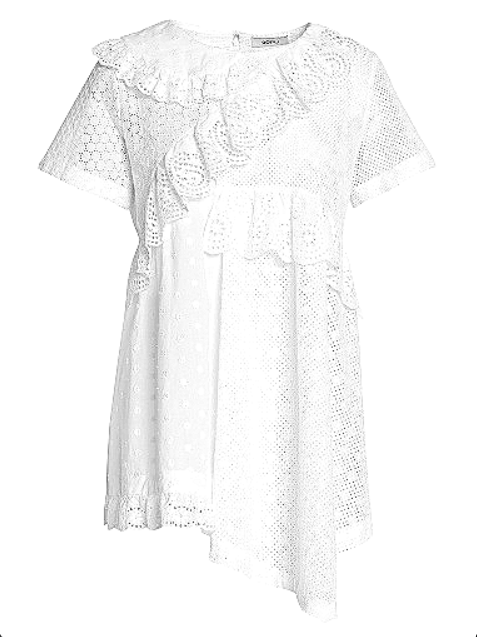
\includegraphics[width = 1.0in]{sharpened_image.png}} &
\subfloat[Canny Edges after Sharpening]{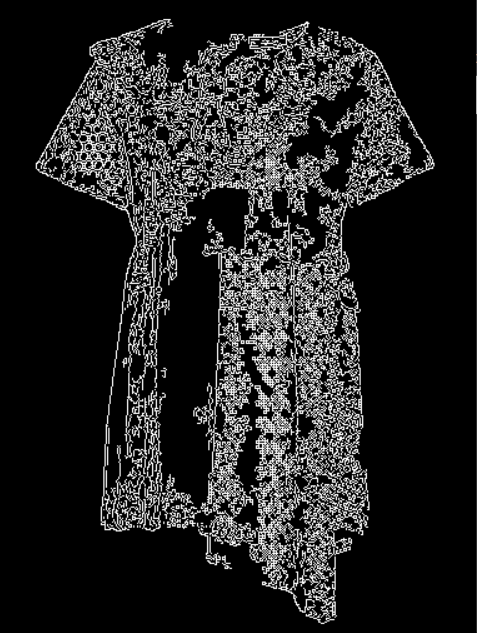
\includegraphics[width = 1.0in]{sharpened_canny_edges.png}} &
\subfloat[Dilated Canny Edges after Sharpening]{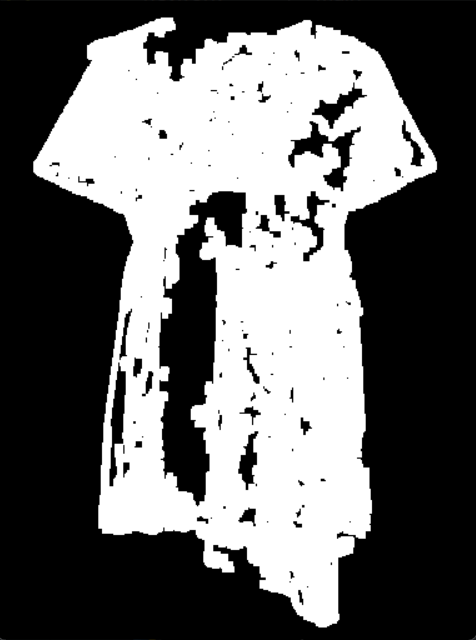
\includegraphics[width = 1.0in]{dilated_sharpened_canny_edges}} &
\subfloat[Mask after Sharpening]{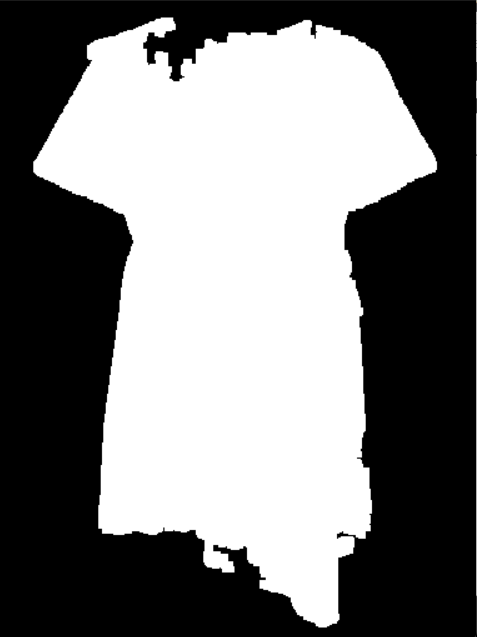
\includegraphics[width = 1.0in]{sharpened_mask.png}} \\
\subfloat[Mask after Median Blur Filter]{
\includegraphics[width = 1.0in]{median_blur_mask.png}} \\
\end{tabular}
\caption{Cloth Mask Extraction Pipeline}
\end{figure}


\subsection{Cloth Retrieval}

The goal of this module is to match a real-world example of a garment item to the same or similar item in an online shop. We take inspiration from Exact-Street-to-Shop approach that makes two interesing points:
\begin{itemize}[noitemsep]
	\item mixing up the geometric/perceptual and the deep-learning works pretty well;
	\item tackle the cloth-matching problem as a binary classification (match or not).
\end{itemize}

We built a reference repository of in-shop cloth items, using the cloth-only images in DressCode. For each cloth item we extract a new feature representation following these steps:
\begin{outline}
 \1 for each image channel (DressCode images are in the RGB format):
   \2 run ORB algorithm to compute the keypoints and the corresponding descriptors;
   \2 compute the histogram on the 256 different color levels;
   \2 concatenate all the values in a 1D tensor;
 \1 concatenate all the channel tensors in a 1D tensor and save it.
\end{outline}

The noise-clean desidered cloth image is fed to a sub-module that detects the cloth area (as a bounding box), using SCHP. From this area is extracted a new feature representation (query-feature) following the same steps presented for the cloth-only images. Then, the comparisons are performed:
\begin{outline}
\1 for each in-shop cloth:
	\2 concatenate the query-feature with the in-shop cloth feature in a 1D tensor;
	\2 fed the tensor to the deep neural network;
	\2 save the similarity (match) score.
\1 sort and select the $k$-best matched in-shop clothes according to the matching-score given by the network. 
\end{outline}

The deep neural network we designed is composed by:
\begin{itemize}
	\item{a linear layer: it performs the embedding of the input tensor;}
	\item{an encoder layer: it performs the representation conversion of the given embedding}
	\item{a linear layer and softmax: it converts the output of the transformer encoder in two probability scores (matching and no-matching.}
\end{itemize}
The higher probability score determines the classification result of the query-feature. We tried two different encoder layers: sequence of linear layers and transformer encoder layer, as depicted in the figure \ref{fig:cloth-retrieval-net}.

\begin{figure}[h]
\centering
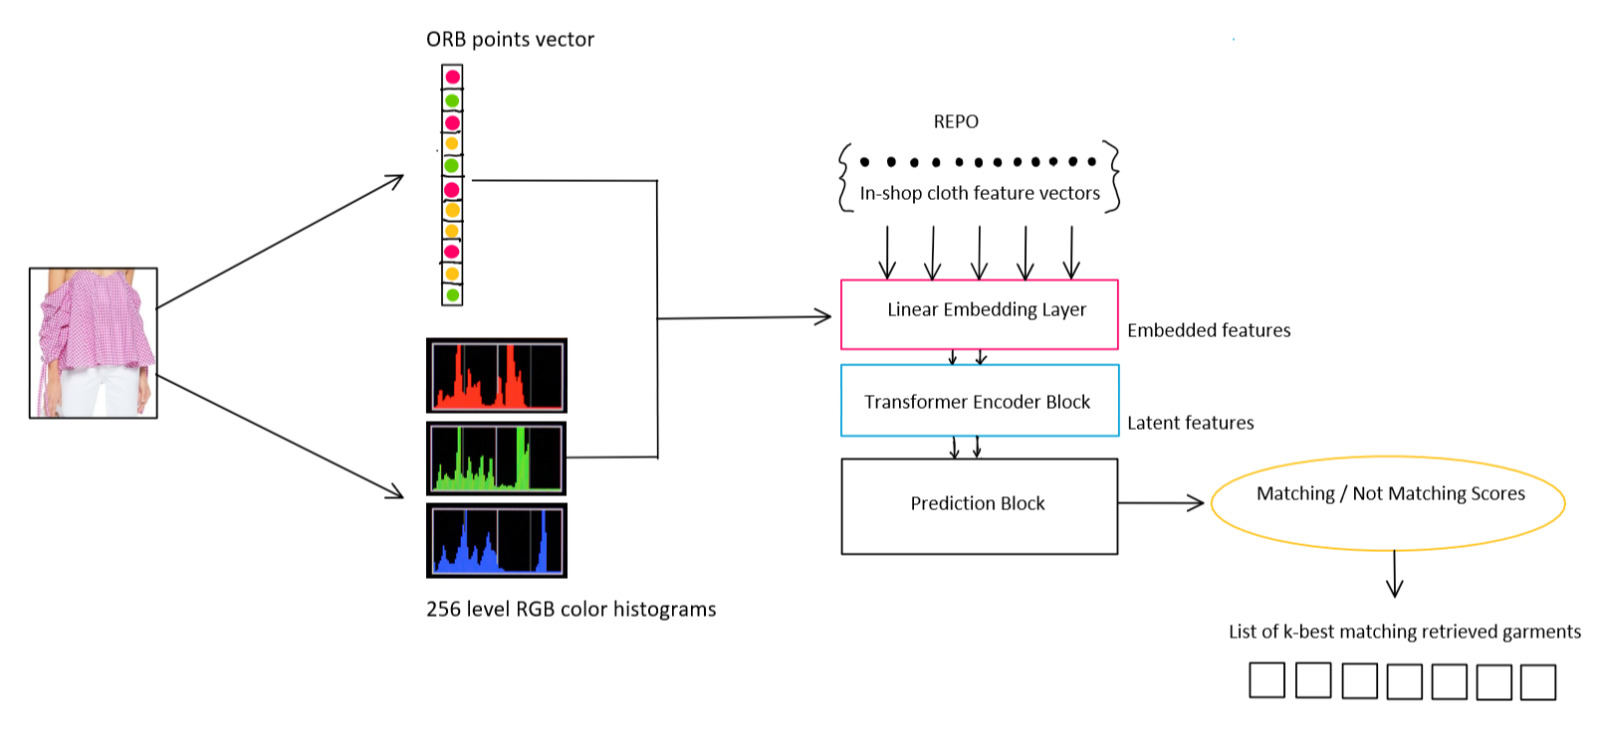
\includegraphics[width=\linewidth,height=110mm,keepaspectratio]{retrieval_net_cv}
\caption{Transformer-based Retrieval Network.}
\label{fig:cloth-retrieval-net}
\end{figure}



To train this network, we used the cross-entropy loss. More in the \ref{retrieval-training} section.



\subsection{Data-Preprocessing and Data-Loading Adaptation}
In orderd to perform the virtual-try-on task we were inspired by CP-VTON+ \cite{CP-VTON+} public repository, but it was deprecated. Thankfully, we found a fixed and updated version \cite{ARajgor}.


Once we checked the proper functioning of the architecture on the VITON dataset we had to adapt the process of dataloading because the Dresscode dataset was different:
\begin{itemize}
\item it lacked binary cloth masks and binary person masks;
\item the body parts segmentation on which the module was originally trained used different labeling technique: the body parts were mapped in different classes;
\item the size of the dataset was way too big (70 GB) for our purposes, therefore we could not use the official training-test split list, and we had to re-sample and resize the images.
\end{itemize}

We first resized the images using \textit{preprocessing/dataset\_resize.py} script. 
After that, we ran the cloth mask generation script, saving only the samples with an acceptable mask (\textit{preprocessing/cloth\_mask\_generator.py}).
We then ran the body shape mask extractor (\textit{preprocessing/mask\_from\_dataset.py}).
We also needed a script that adapted DressCode keypoints format to the Openpose json format accepted by the original dataloader. (\textit{preprocessing/json\_conversion.py})
The last step was to subsample the original dataset and re-create the train-test list text file used to load it. All the procedure is in (\textit{preprocessing/dataset\_subsample.py} and \textit{preprocessing/dress\_code\_train\_test\_txt\_gen.py}).

The resulting dataset contained 11.959 upper-body samples and 24.309 dresses samples, in 512x384 resolution. 

We also modified the Dataset class used by the dataloader, changing some file names conventions and creating a new label map dictionary to adapt the DressCode SCHP based body parts segmentation masks to the system. See more in \textit{network/cp\_dataset\_modified.py} (Dictionary name: \textit{DressCode\_labelmap\_g}).

\subsection{Warping Module}
We follow the warping module proposed in CP-VTON+ \cite{CP-VTON+}.
This module transforms the input try-on garment $c$ into a warped image of the same item that matches the body pose $p$ and shape $m$. As warping function we use a thin-plate spline (TPS) geometric transformation, which is commonly used in virtual try-on models.  Inside this module, we aim to learn the correspondence between the inputs $(c, p, m)$ and the set of parameters $\theta$ to be used in the TPS transformation. Intuitively, the TPS fits a surface (try-on garmet) through points (feature regression output points) minimizing an energy function. Formally, it is a poli-harmonic spline function which maps a set of points $(x,y)$ on their correspondences $(x',y')$ sampled from input images. Under these terms, the warping module aims to learn how to perform such transformation.

As depicted in figure \ref{fig:GMM_MODULE}, the module extracts an encoded representation of the try-on garment $c$ and an encoded representation of the person representation through two separate convolutional networks.
Then, it is computed a correlation map between these representations.
This correlation map is used to predict the spatial transformation parameters $\theta$ corresponding to the $(x,y)$-coordinate offsets of TPS anchor points. 

To train this network, we used the following loss:
\begin{equation}
L(\theta) = \lambda_1 \cdot L_1(c_{warped}, I_{c_t}) + \lambda_{reg} \cdot L_{reg} ;
\end{equation} 
where:
\begin{itemize}[noitemsep]
	\item{$L_1$ is the $L_1$ pixel-wise loss between the warped result and the ground truth;} 
	\item{$L_{reg}$ is a regularization term applied to the anchor points (that represents the warping grip), in order to avoid excessive warping distortions.}
\end{itemize}
 

\begin{figure*}[h]
\centering
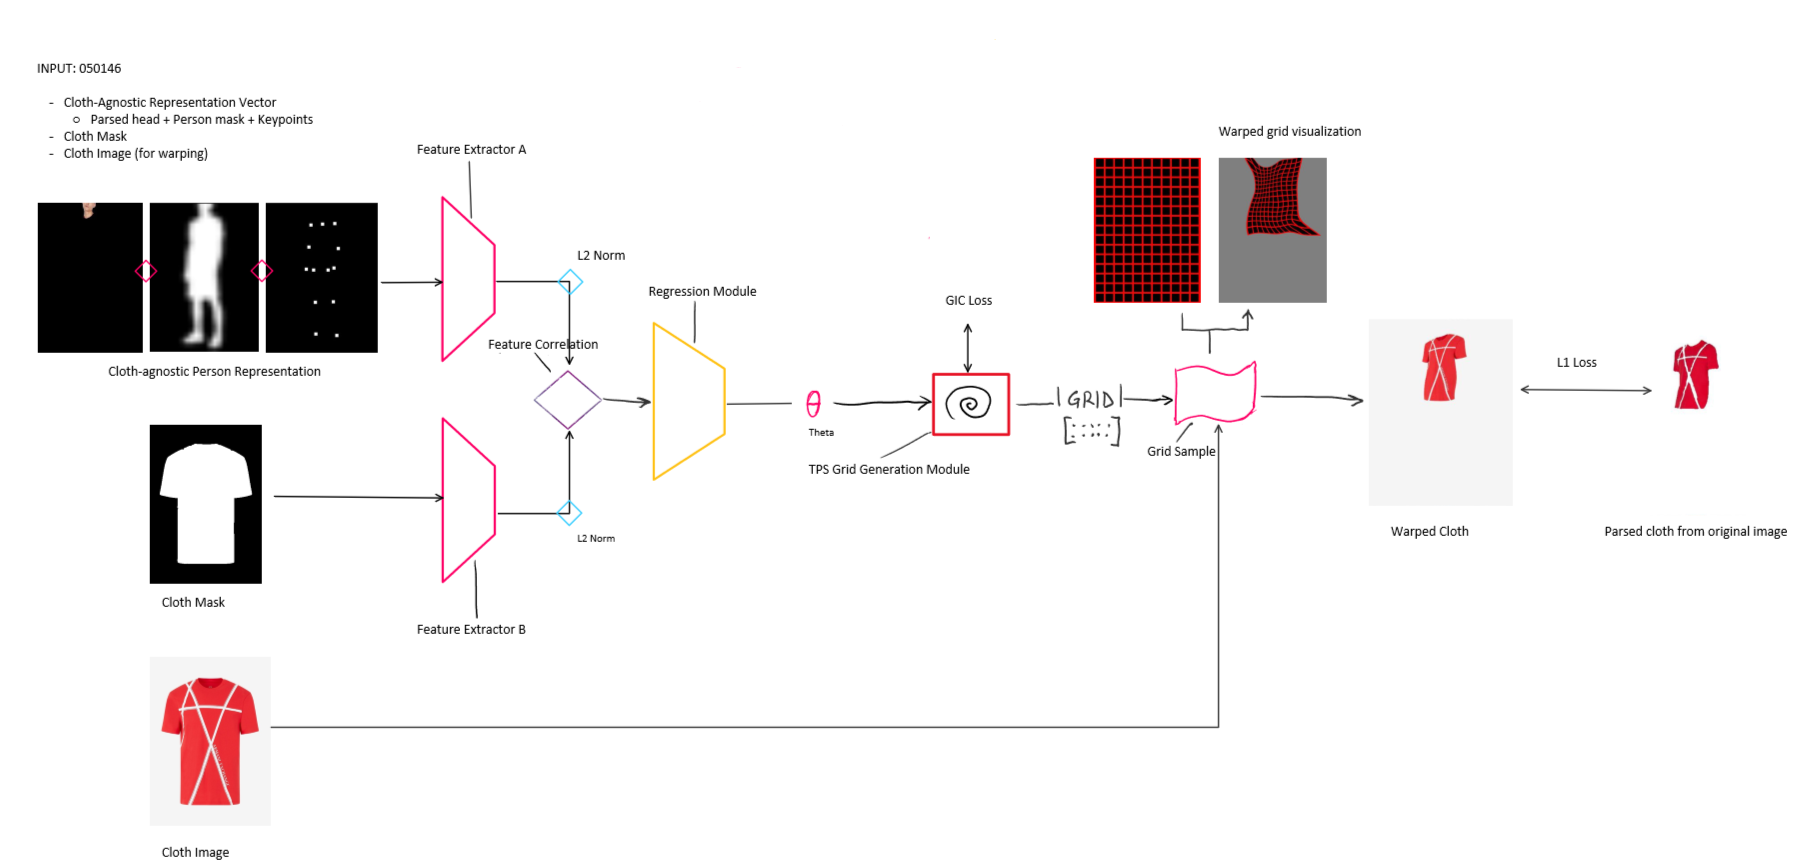
\includegraphics[width=\linewidth,height=100mm,keepaspectratio]{GMM_MODULE}
\caption{Geometric Warping Module Overall Architecture}
\label{fig:GMM_MODULE}
\end{figure*}



\subsection{Generative Module}
This module aims at fitting the warped garment on the target person. Previous works like CP-VTON and CP-VTON+ directly concatenate the person image $p$, the warped clothing image
$\hat{c}$, and the warped clothing mask image $\hat{cm}$ . 

\begin{figure}[h]
\centering
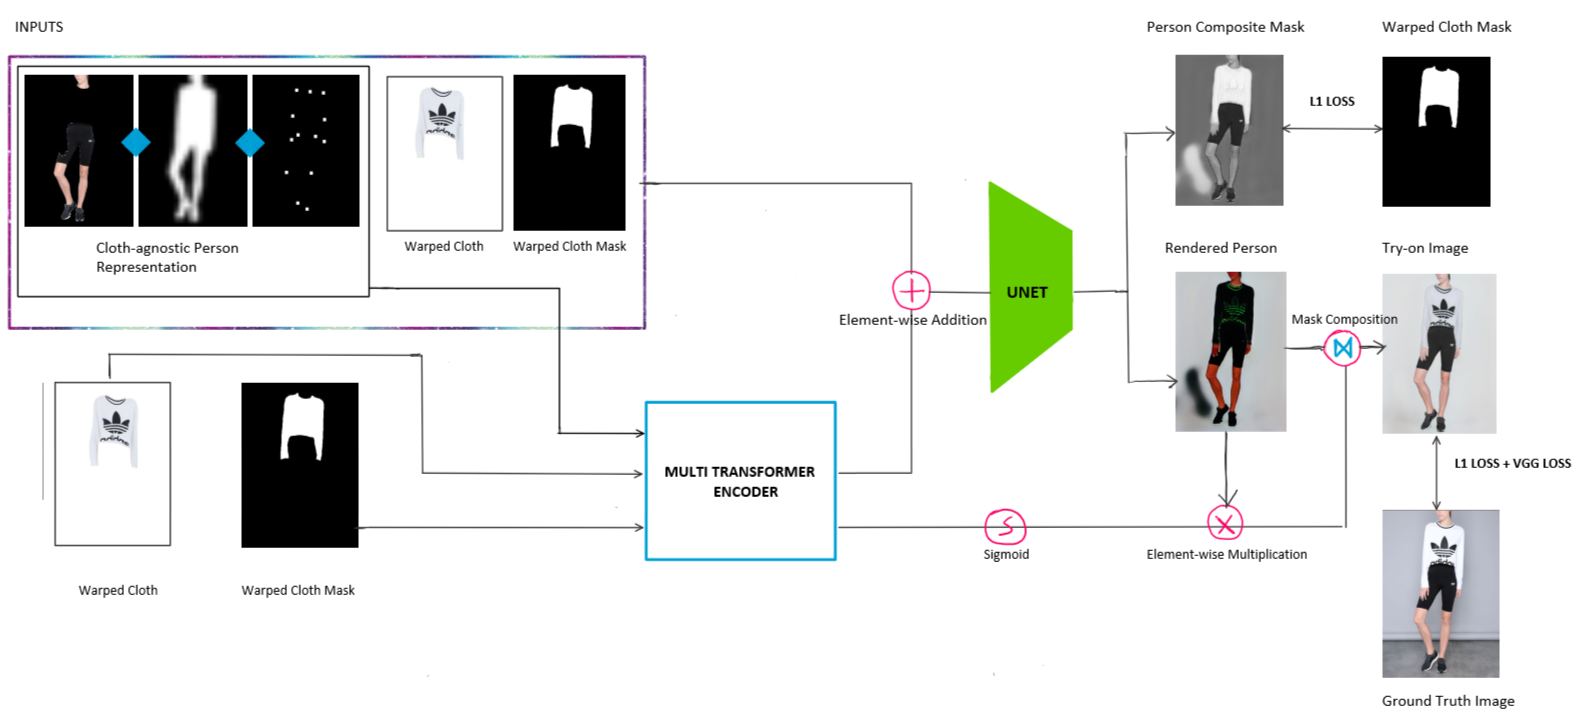
\includegraphics[width=\linewidth,height=100mm,keepaspectratio]{TOM_MODULE}
\caption{Try-On Module Overall Architecture}
\label{fig:TOM_MODULE}
\end{figure}

Then the concatenated input is sent to a UNet \cite{u-net} to generate a composition mask $M_o$ and a rendered person image $I_R$. The main limitation of this approach is the inability of the convolution operator to model global long-range dependences. For this reason, we follow the CIT \cite{CIT} approach that leverage the Transfomer-based architecture and cross-modal attention mechanism that are able to capture the dependence among these three input images.


As shown in the figure \ref{fig:cit_architecture}, the three inputs goes through the patch embedding, for making the image data compatible.  Then each goes through a 1D temporal convolution to ensure the relation modeling of each element with its neighbor elements. Then the Interactive-Transformer II is utilized for modeling the global long-range correlation. The output $X_{out-II}$ of Interactive Transformer II is obtained after a linear projection and a reshape operation. Then $X_{out-II}$ is utilized for two proposes; one is to activate the important region of the overall input by adding $X_{out-II}$ to $I(p,\hat{c},\hat{cm})$; another is to guide the final mask composition as follows:

\begin{equation}
  \begin{aligned}
    I_{R}^{global} = sigmoid(X_{out-II}) \times I_R, \\
I_o = M_o \times \hat{c} + (1 - M_o) \times I_{R}^{global}
  \end{aligned}
\end{equation}

where $\times$ represents the element-wise multiplication and $sigmoid$ indicates the sigmoid activation function.

\FloatBarrier
\begin{figure}[h]
\centering
\begin{subfigure}{0.7\linewidth}
  \centering
  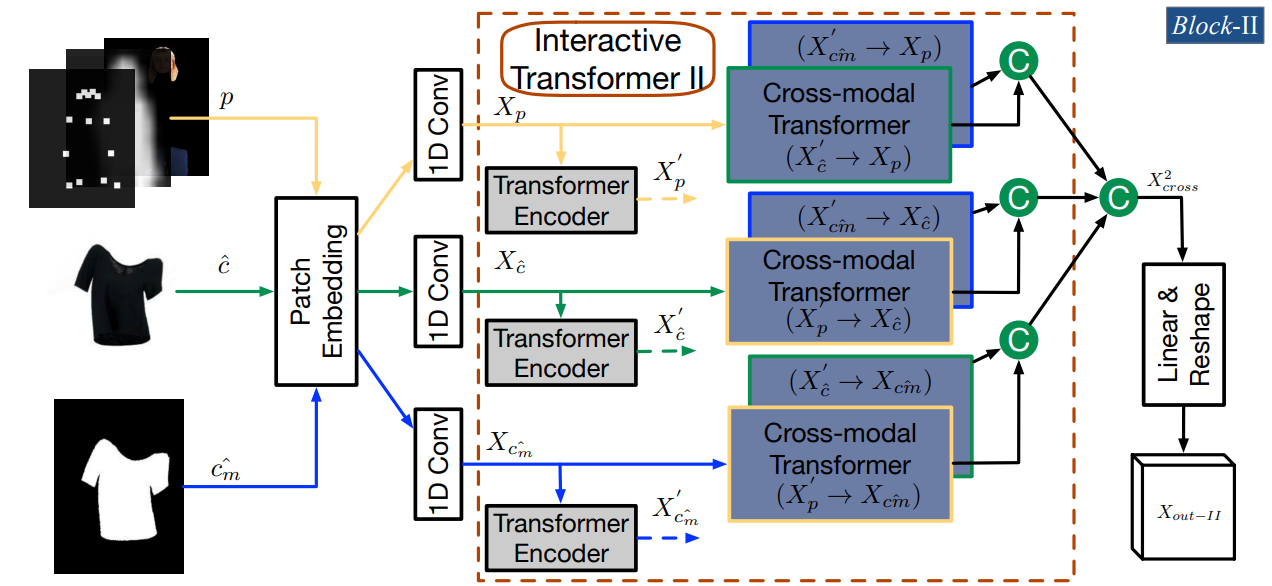
\includegraphics[width=1\linewidth]{cit_reasoning_block}
  %\caption{CIT Reasoning Block architecture, also called Interactive-Transformer II}
  \label{fig:sub1}
\end{subfigure}%
\begin{subfigure}{0.3\linewidth}
  \centering
  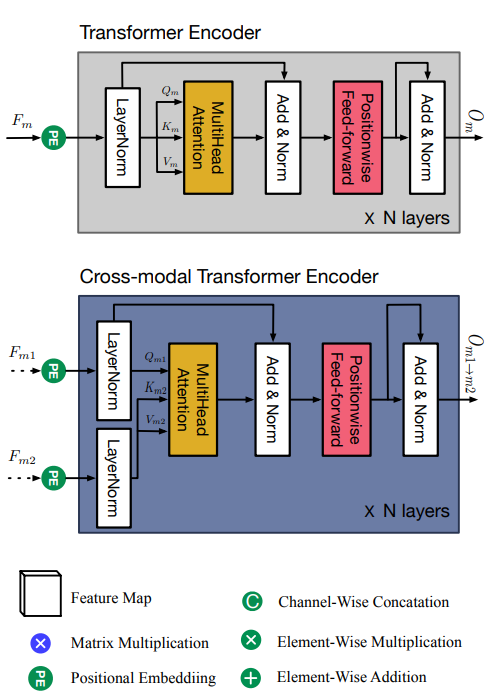
\includegraphics[width=1\linewidth]{cit_reasoning_block_2}
  %\caption{Legend}
  \label{fig:sub2}
\end{subfigure}
\caption{On the left: CIT Reasoning Block architecture, also called Interactive-Transformer II. On the right: the Transformer Encoder and Cross-Modal Transformer Encoder architetures and a legend of symbols.}
\label{fig:cit_architecture}
\end{figure}
\FloatBarrier

\subsection{Training}
We performed five training steps. GMM module for upper-body and dresses garments, TOM module with CIT and TOM module without CIT for upper-body garments, and TOM module without CIT for dresses garments. We evaluated results by IoU measure for the warping step, and by SSIM, FID and MSE for the generative step.
\subsubsection{Setup}
In all experiments, we use $L1 = $vgg = 1. We trained GMM Modules for 315.000 steps batch size 4. We use Adam optimizer with $\beta_1 = 0.5$ and $\beta_2 = 0.999$. Learning rate is first fixed at 0.0001 for 100K steps and then linearly decays to zero for the remaining steps.

Due to the heavy computational load of the CIT reasoning block, the upper-body generative modules were trained for 50.000 steps only. To have an idea, without CIT block one training step required about 1 second, with CIT block it required 10 seconds. Batch size and optimizer options are the same.
We were able to supervise the training procedure by Tensorboard tool.

\subsubsection{Upper body Training}

Some insight into the Geometric Matching Module.

\begin{figure}[h]
\centering
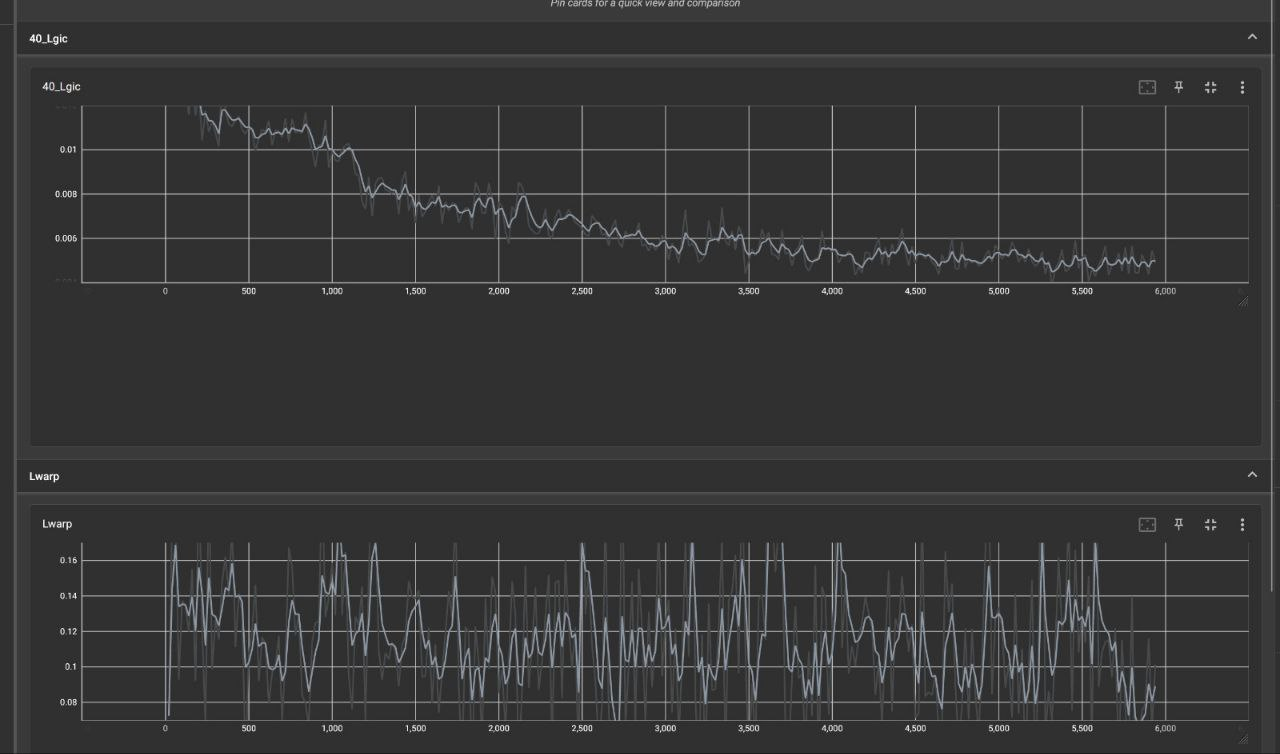
\includegraphics[width=\linewidth,height=60mm,keepaspectratio]{losses}
\caption{GMM Gic and Warp Losses evolution}
\label{fig:TOM_MODULE}
\end{figure}

\begin{figure}[h]
\centering
\begingroup

\setlength{\tabcolsep}{25pt} % Default value: 6pt
\renewcommand{\arraystretch}{1.5} % Default value: 1

\begin{tabular}{cccc}
\subfloat[In-shop cloth]{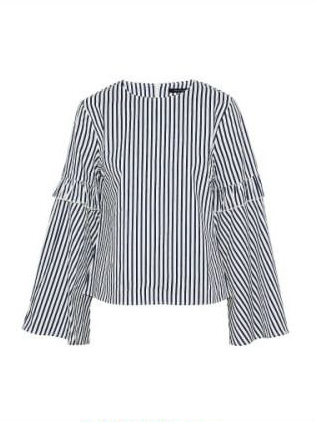
\includegraphics[width = 1.0in]{clothw.png}} &
\subfloat[Warped cloth]{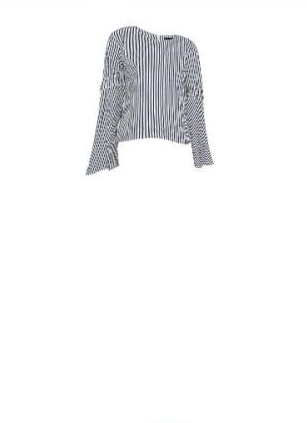
\includegraphics[width = 1.0in]{clothwarp.png}} &
\subfloat[Ground truth worn cloth]{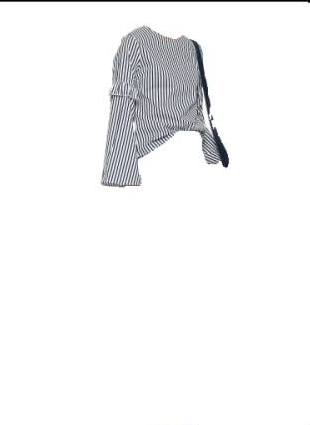
\includegraphics[width = 1.0in]{warpgt.png}} \\
\subfloat[Warped grid]{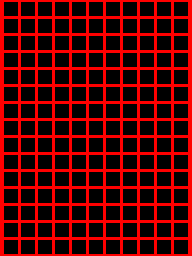
\includegraphics[width = 1.0in]{grid.png}} &
\subfloat[Warped cloth over image]{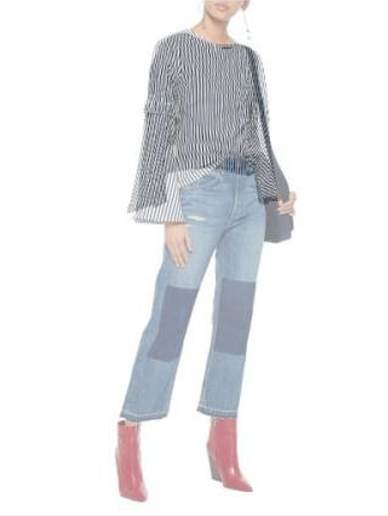
\includegraphics[width = 1.0in]{wornboh.png}} &
\subfloat[Ground truth person image]{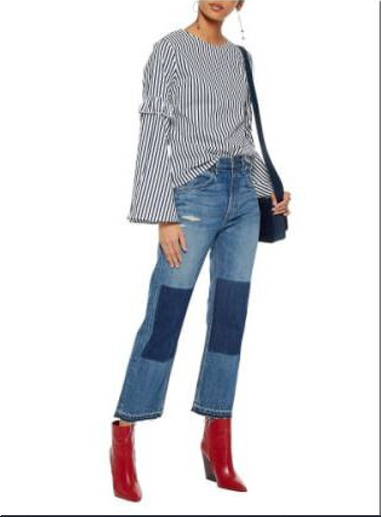
\includegraphics[width = 1.0in]{gtimage.png}} \\
\end{tabular}

\endgroup

\caption{Example of the warping stage of an in-shop cloth image over a paired person image}
\end{figure}

We trained the network with 11.411 training images and tested it on 1.196 test images.
Some comparison between CIT and baseline generated images on test-set:

\begin{table}[h]
        \centering
        \begin{tabular}{ccccc}
            With CIT Block & 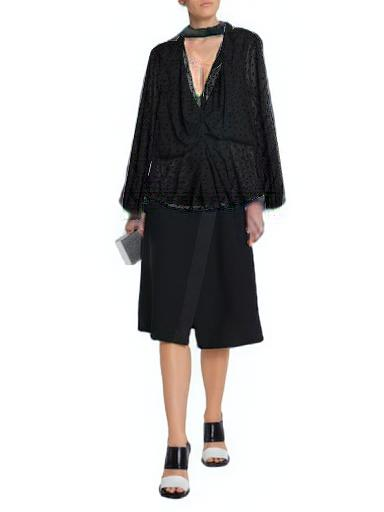
\includegraphics[width = 1.2in]{cit_000826_0.jpg} & 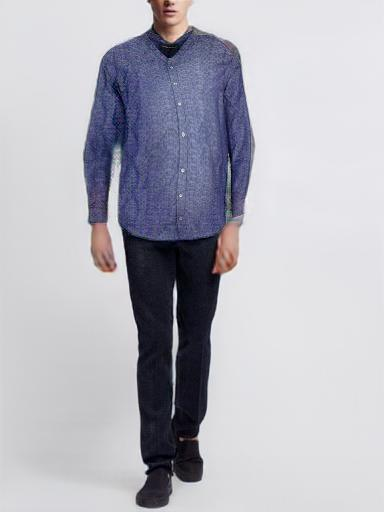
\includegraphics[width = 1.2in]{cit_001820_0.jpg} & 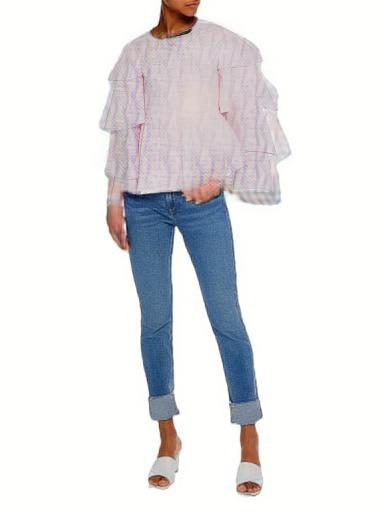
\includegraphics[width = 1.2in]{cit_002566_0.jpg} \\
            Without CIT Block & 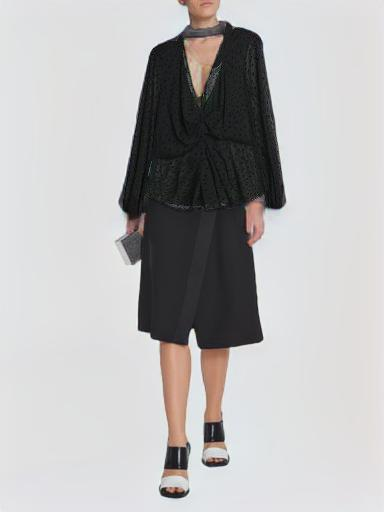
\includegraphics[width = 1.2in]{000826_0.jpg} & 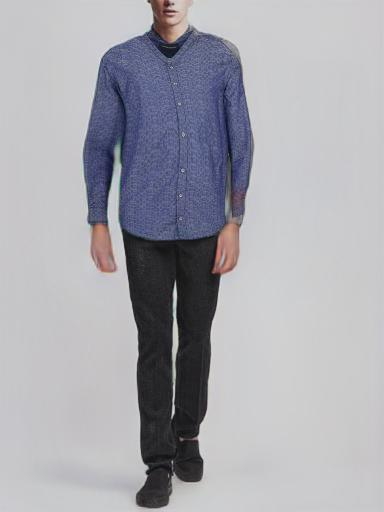
\includegraphics[width = 1.2in]{001820_0.jpg} & 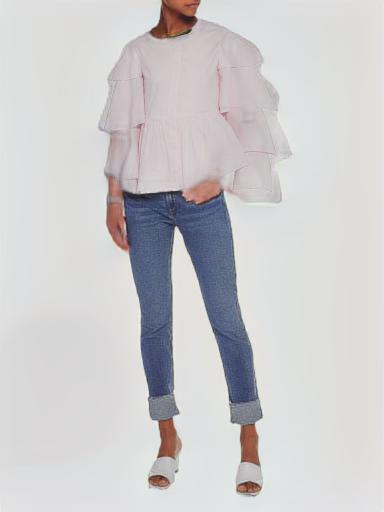
\includegraphics[width = 1.2in]{002566_0.jpg}\\
        \end{tabular}
        \caption{Comparison between Generation with and without CIT block}
        \label{tbl:table_of_figures}
\end{table}


\subsubsection{Dresses Training}

Training on the Dresses category was only performed using the baseline version of the generative network to save computational time. We trained the network on 24.309 images for 200.000 steps for the warping module and 100.000 steps for the generative module, and tested it on 2.431 images.


\begin{figure}[h]
\centering
\begin{tabular}{cccc}
{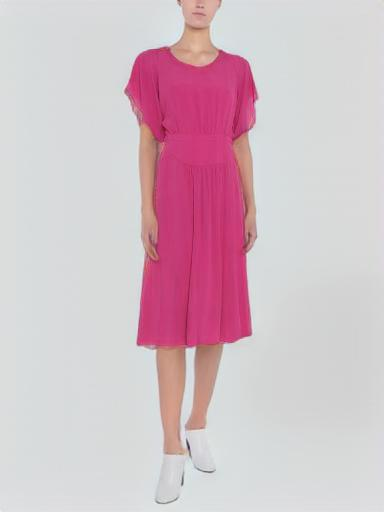
\includegraphics[width = 1.2in]{021651_0.jpg}} &
{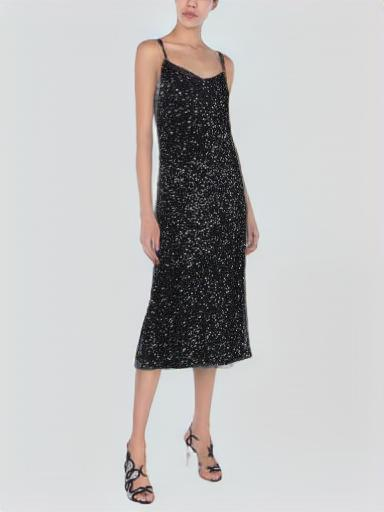
\includegraphics[width = 1.2in]{020942_0.jpg}} &
{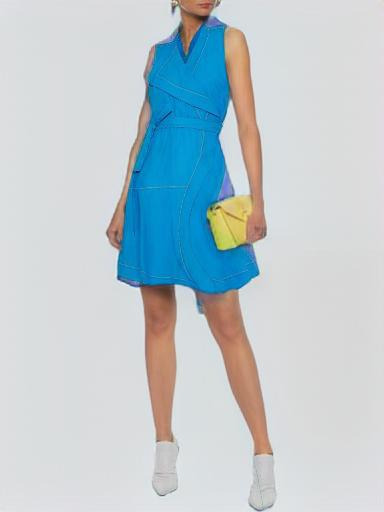
\includegraphics[width = 1.2in]{035858_0.jpg}} &
{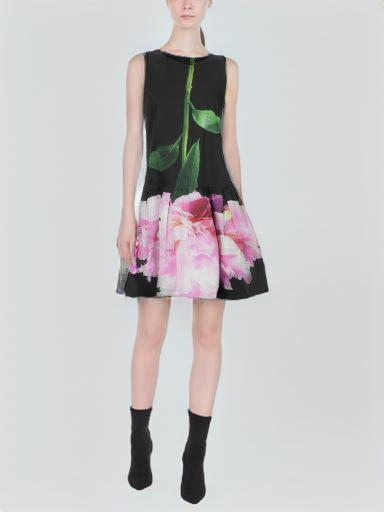
\includegraphics[width = 1.2in]{041678_0.jpg}} \\
\end{tabular}

\caption{Some examples of test Dresses generated images.}
\end{figure}



\subsubsection{Final Experiment Results}
We computed some measures between our results and other available benchmarks from other papers. Due to the different test set and the different number of steps, a comparison between our work and other official publication results is misleading. The only fair comparison is between the two upper-body generative results, which are both trained on the same data and the same number of steps (50.000). The results show that the CIT block indeed increase the generative image performance. The measures are computed on paired image couples, but we also performed an unpaired cloth-person test set generation. Scripts can be found in the \textit{measures} folder.

\begin{figure}[h]
\centering
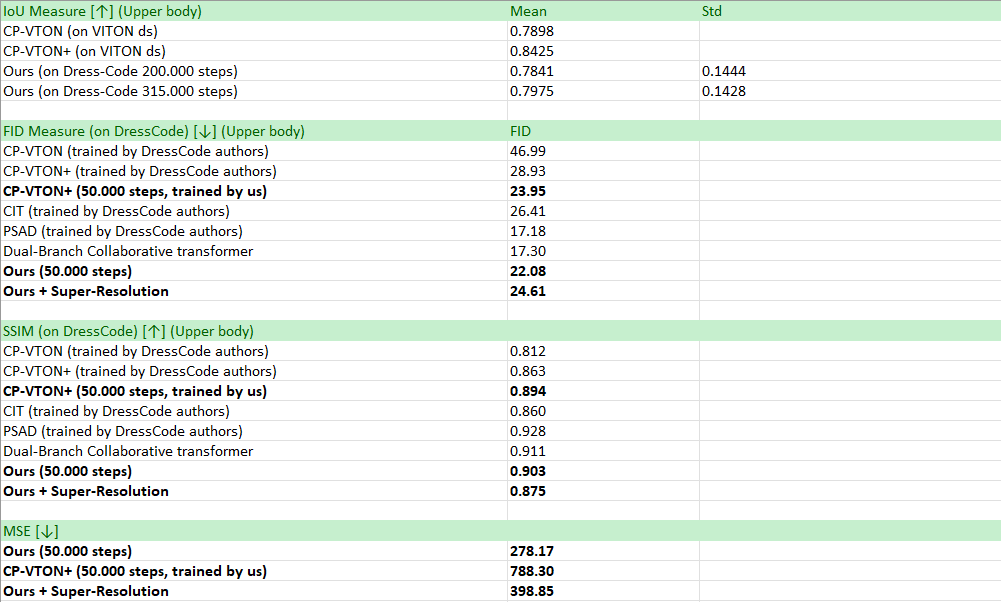
\includegraphics[width=\linewidth,height=110mm,keepaspectratio]{measures}
\caption{Experimental results}
\label{fig:Measures}
\end{figure}


\subsubsection{Cloth-Retrieval-Net Training}
\label{retrieval-training}

To train this network, we used the cross-entropy loss, applying the dropout regularization technique ($p=0.1$).

During training, the network tried to classify both positive examples (the paired couples of worn-cloth and cloth taken) and negative examples (not paired couples). Since the number of potential negative examples was far more the number of positive examples, we used data augmentation to creating synthetic positive examples from existing one: we applyed multivariate gaussian noise to the feature representations.

We compared two architectures with similar structure:
\begin{itemize}[noitemsep]
	\item{fully linear architecture: it is composed only by linear layers;}
	\item{transformer-based architecture: it is composed by linear and a transformer encoder layers.}
\end{itemize}
The figure \ref{fig:cloth-retrieval-results} depicts the obtained results. Furtheremore, we validate our results with human (subjective) evaluation of top-5 ranked results. A person checked the top-5 results of the retrieval for random in-the-wild pictures: if in these retrieved images there was at least an acceptable matching garment, the retrieved was considered succesfull. With a little abuse of notation, we called these results \textit{Top-5 Accuracy}, depicted in the figure \ref{fig:cloth-retrieval-results}.

\begin{figure}[h]
\centering
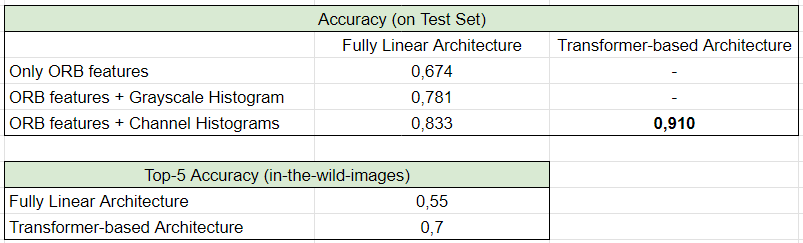
\includegraphics[width=\linewidth,height=110mm,keepaspectratio]{retrieval_metrics}
\caption{Cloth-retrieval results}
\label{fig:cloth-retrieval-results}
\end{figure}



\subsection{Post-Processing and Super-Resolution}

The final step of the pipeline consists in applying an upscaling to the generated image, to obtain both an higher resolution and a correction of some generative defects. The upscaling is done through a recently released architecture named \textit{ControlNet} \cite{controlnet}. ControlNet is a neural network structure to control diffusion models by adding extra conditions. You can choose a StableDiffusion base model and through some prompt an input image, the generation is forced to follow the basic structure of the input image. There are various models trained for example to generate images from edges maps, from depth maps and so on. We chose the \textit{tile} architecture \cite{tile}, trained to perform a realistic upscaling. Our positive prompt was set to $$prompt = "best quality, clothes, garment, model, shop, upper clothes"$$ and the negative one to $$prompt = "blur, lowres, bad anatomy, bad clothes, bad hands, cropped, worst quality,$$
 $$fading, glitch, robot, tech, high saturation, medieval"$$
The complete script is \textit{super-resolution/controlNet.py}

\begin{table}[h]
        \centering
        \begin{tabular}{ccccc}
            Original & 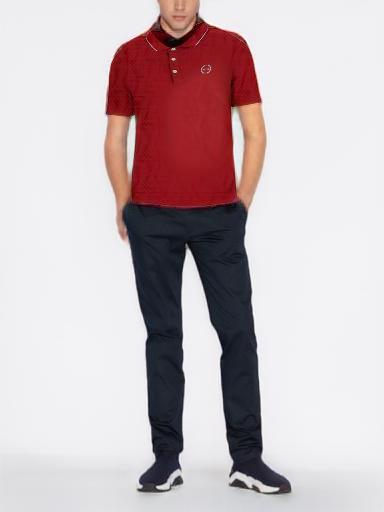
\includegraphics[width = 1.5in]{000229_0cit.jpg} & 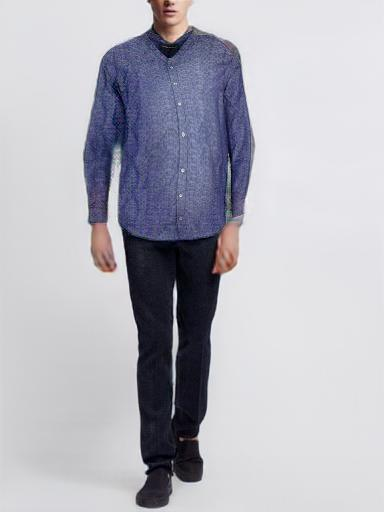
\includegraphics[width = 1.5in]{cit_001820_0.jpg} & 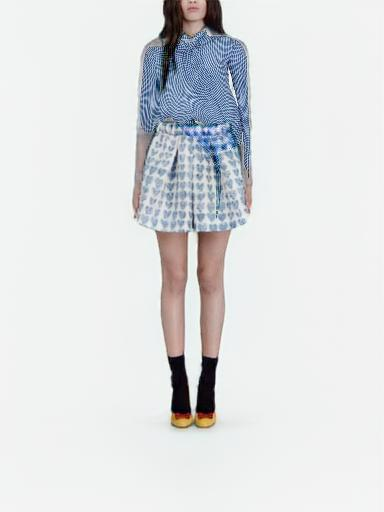
\includegraphics[width = 1.5in]{000380_0cit.jpg} \\
            With Super-Resolution & 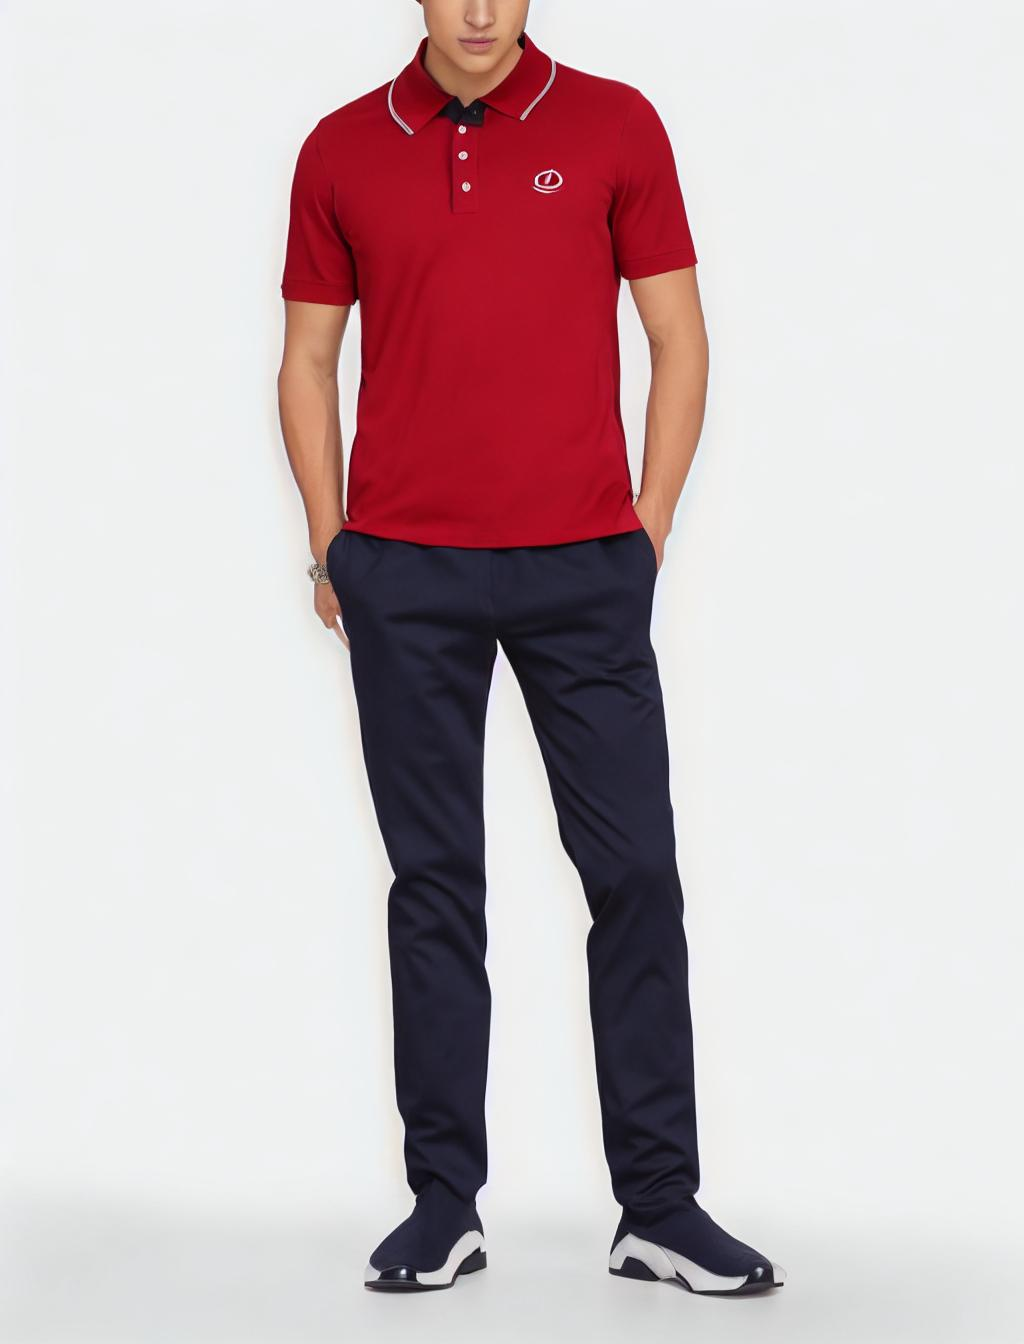
\includegraphics[width = 1.5in]{000229_0sr.jpg} & 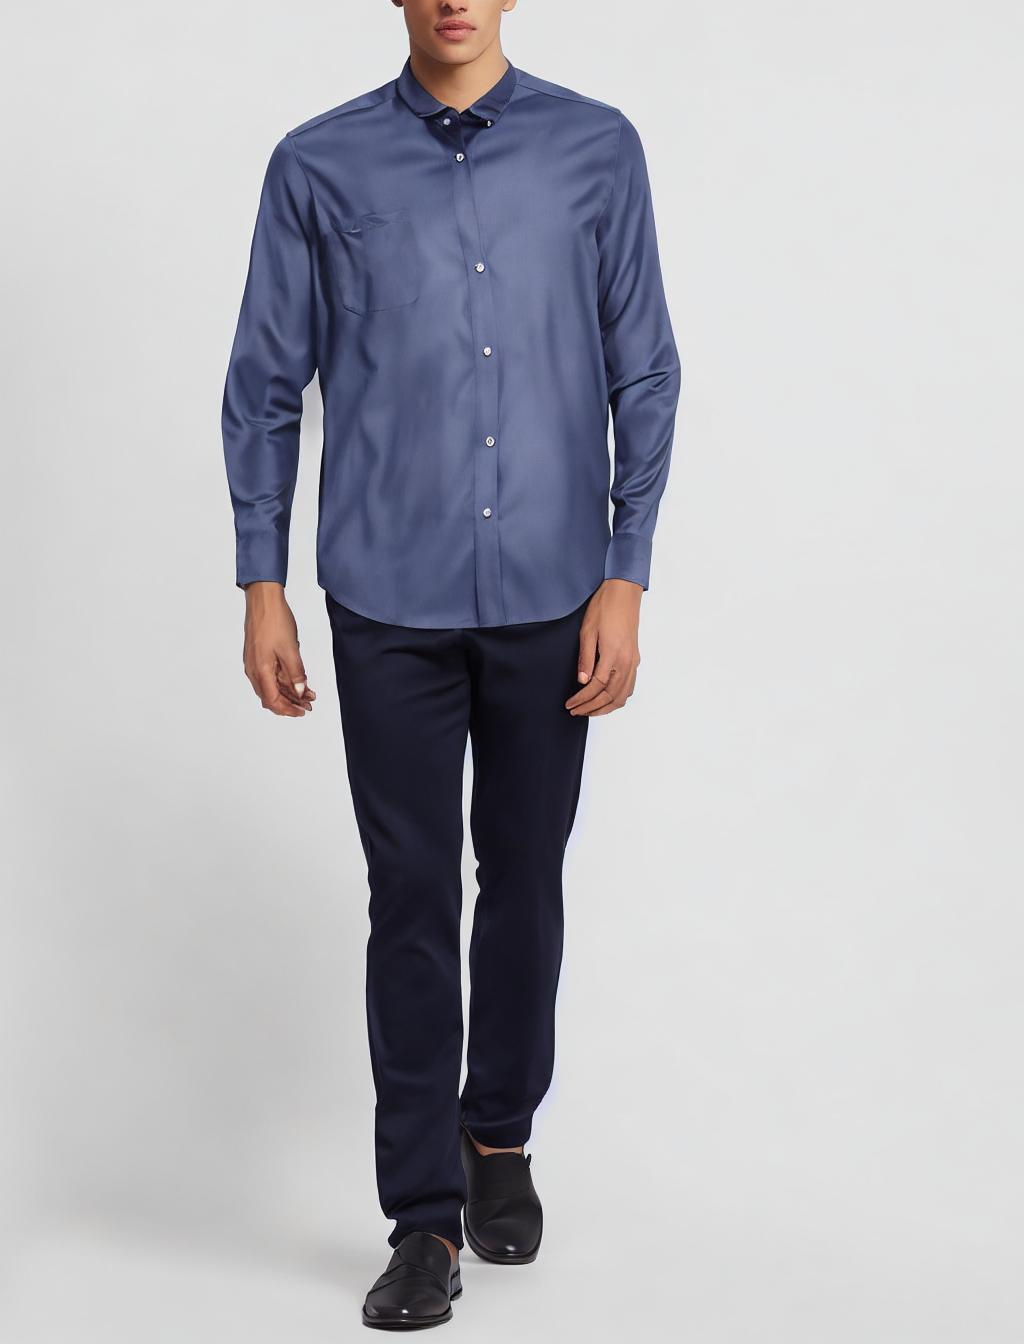
\includegraphics[width = 1.5in]{001820_0sr.jpg} & 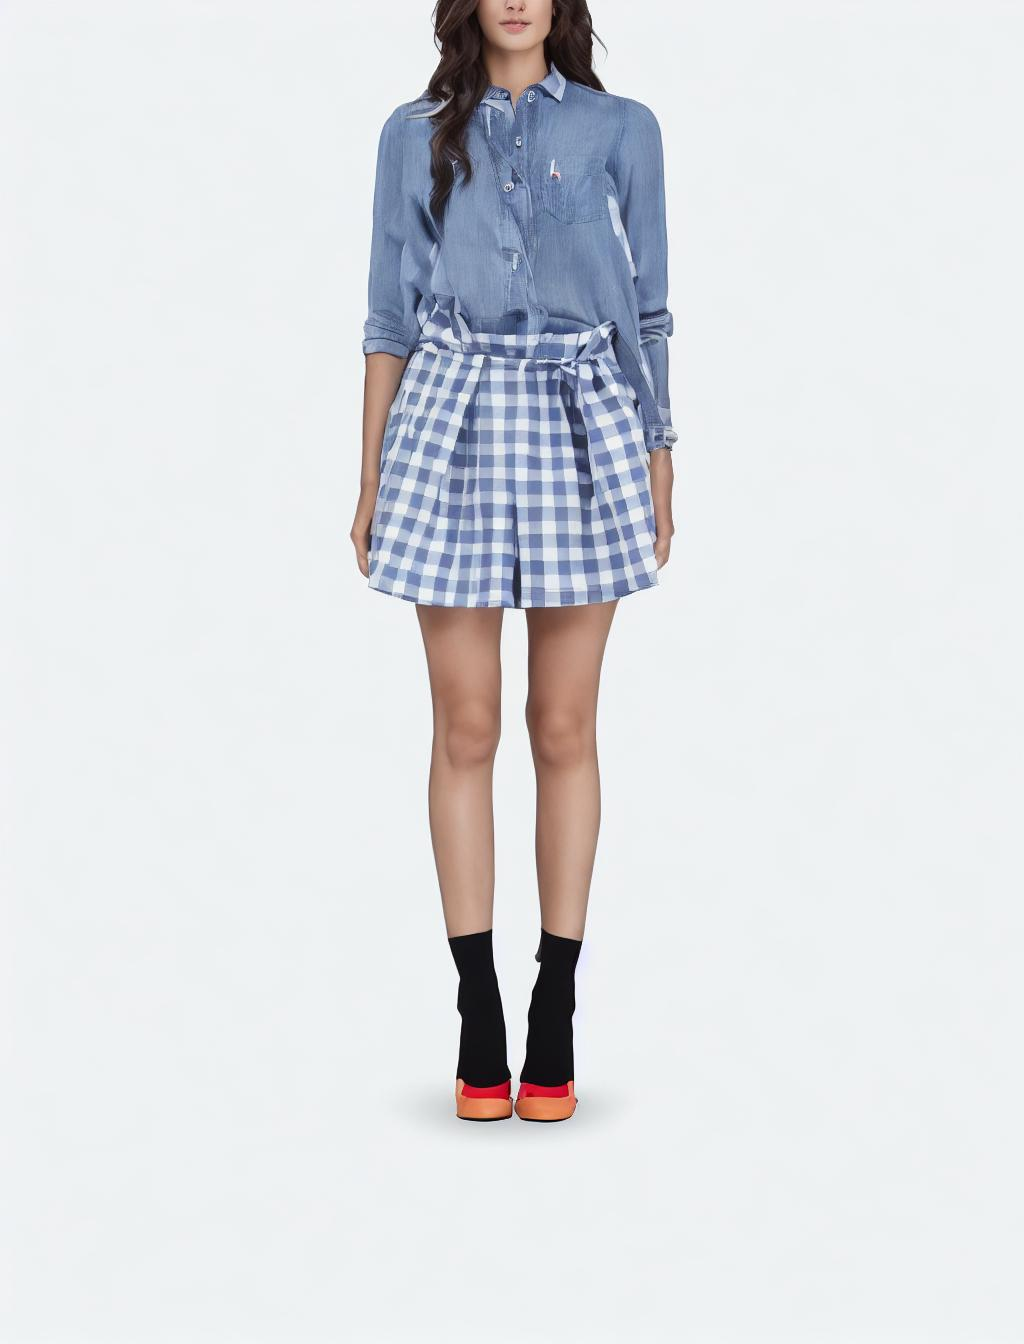
\includegraphics[width = 1.5in]{000380_0sr.jpg}\\
        \end{tabular}
        \caption{Comparison between generated images and generated images after Super-Resolution}
        \label{tbl:table_of_figures}
\end{table}

\begin{figure}[h]
\centering
\begin{tabular}{ccccc}
\subfloat[Input image]{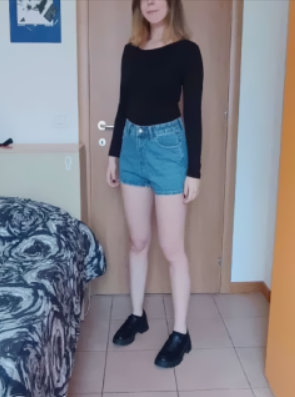
\includegraphics[width = 1.2in]{boh1.png}} &
\subfloat[No background image]{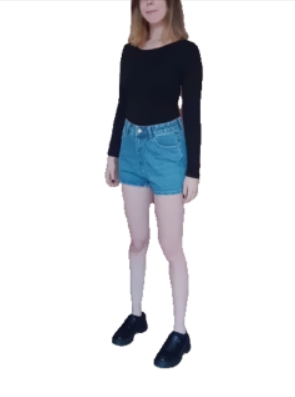
\includegraphics[width = 1.2in]{boh2.png}} &
\subfloat[In-shop cloth]{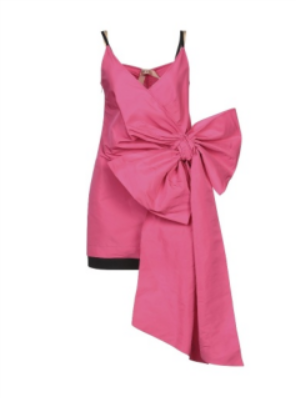
\includegraphics[width = 1.2in]{boh3.png}} &
\subfloat[Try-on image]{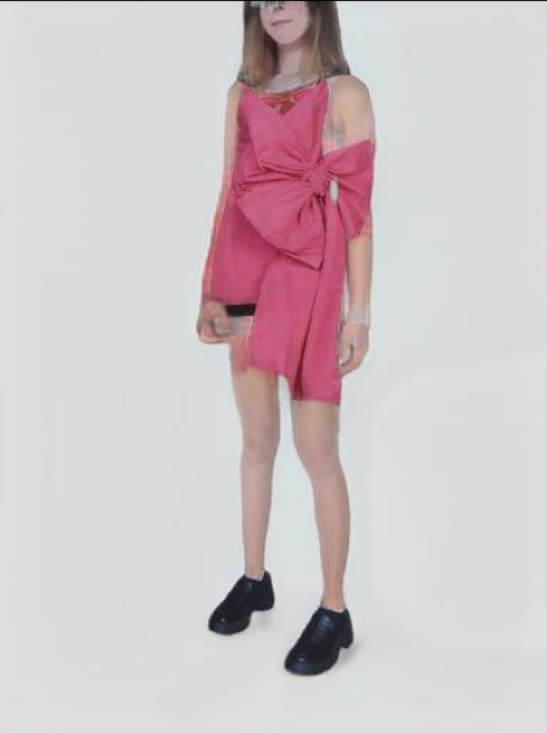
\includegraphics[width = 1.2in]{boh4.png}} &
\subfloat[Super-resolution image]{\includegraphics[width = 1.2in]{boh5.png}} \\
\end{tabular}

\caption{Final example of VTON starting from a in-the-wild image}
\end{figure}



